%%%%%%%%%%%%%%%%%%%%%%%%%%%%%%%%%%%%%%%%%
% Beamer Presentation
% LaTeX Template
% Version 1.0 (10/11/12)
%
% This template has been downloaded from:
% http://www.LaTeXTemplates.com
%
% License:
% CC BY-NC-SA 3.0 (http://creativecommons.org/licenses/by-nc-sa/3.0/)
%
%%%%%%%%%%%%%%%%%%%%%%%%%%%%%%%%%%%%%%%%%

%----------------------------------------------------------------------------------------
%    PACKAGES AND THEMES
%----------------------------------------------------------------------------------------

\documentclass{beamer}

\mode<presentation> {

% The Beamer class comes with a number of default slide themes
% which change the colors and layouts of slides. Below this is a list
% of all the themes, uncomment each in turn to see what they look like.

%\usetheme{default}
%\usetheme{AnnArbor}
%\usetheme{Antibes}
%\usetheme{Bergen}
%\usetheme{Berkeley}
%\usetheme{Berlin}
%\usetheme{Boadilla}
%\usetheme{CambridgeUS}
%\usetheme{Copenhagen}
%\usetheme{Darmstadt}
%\usetheme{Dresden}
%\usetheme{Frankfurt}
%\usetheme{Goettingen}
%\usetheme{Hannover}
%\usetheme{Ilmenau}
%\usetheme{JuanLesPins}
%\usetheme{Luebeck} *
%\usetheme{Madrid} *
%\usetheme{Malmoe}
%\usetheme{Marburg}
%\usetheme{Montpellier}
\usetheme{PaloAlto}
%\usetheme{Pittsburgh}
%\usetheme{Rochester}
%\usetheme{Singapore}
%\usetheme{Szeged}
%\usetheme{Warsaw}

% As well as themes, the Beamer class has a number of color themes
% for any slide theme. Uncomment each of these in turn to see how it
% changes the colors of your current slide theme.

%\usecolortheme{albatross}
%\usecolortheme{beaver}
%\usecolortheme{beetle}
%\usecolortheme{crane}
%\usecolortheme{dolphin}
%\usecolortheme{dove}
%\usecolortheme{fly}
%\usecolortheme{lily}
%\usecolortheme{orchid}
%\usecolortheme{rose}
%\usecolortheme{seagull}
%\usecolortheme{seahorse}
%\usecolortheme{whale}
%\usecolortheme{wolverine}

%\setbeamertemplate{footline} % To remove the footer line in all slides uncomment this line
%\setbeamertemplate{footline}[page number] % To replace the footer line in all slides with a simple slide count uncomment this line

\setbeamertemplate{navigation symbols}{} % To remove the navigation symbols from the bottom of all slides uncomment this line
}

\usepackage{graphicx} % Allows including images
\usepackage{booktabs} % Allows the use of \toprule, \midrule and \bottomrule in tables
\usepackage[spanish]{babel}
\usepackage[latin1]{inputenc}
%----------------------------------------------------------------------------------------
%    TITLE PAGE
%----------------------------------------------------------------------------------------

\title[Proxy adaptativo]{Proxy adaptativo para protocolos web avanzados} % The short title appears at the bottom of every slide, the full title is only on the title page

\logo{
\includegraphics[height=1cm]{img/logo}}

\author{Pablo Maximiliano Lulic} % Your name
\institute[UNLu] % Your institution as it will appear on the bottom of every slide, may be shorthand to save space
{
Universidad Nacional de Luj�n\\ % Your institution for the title page
\medskip

\includegraphics[height=2cm]{../tesis/img/logo_unlu}
%\textit{mlulic@unlu.edu.ar} % Your email address
}
\date{\number\the\year} % Date, can be changed to a custom date

\begin{document}

\begin{frame}
\titlepage % Print the title page as the first slide
\end{frame}

\begin{frame}
\frametitle{Sumario} % Table of contents slide, comment this block out to remove it
\tableofcontents % Throughout your presentation, if you choose to use \section{} and \subsection{} commands, these will automatically be printed on this slide as an overview of your presentation
\end{frame}

%----------------------------------------------------------------------------------------
%    PRESENTATION SLIDES
%----------------------------------------------------------------------------------------

%------------------------------------------------
\section{Introducci�n}
%------------------------------------------------

\begin{frame}
\frametitle{Introducci�n}

?

\end{frame}

%------------------------------------------------
\section{Crecimiento Web} 
%------------------------------------------------

\begin{frame}
\frametitle{La web de hace a�os}

\textbf{Como eran los sitios hace 14 a�os?}

\begin{itemize}
	\pause \item Sitios sencillos
	\pause \item Poco contenido
	\pause \item Tama�o aproximado de 70kb %ref 40 de la tesis
\end{itemize}

\end{frame}

%------------------------------------------------

\begin{frame}
\frametitle{Sitio de Amazon, a�o 2000}

\begin{figure}
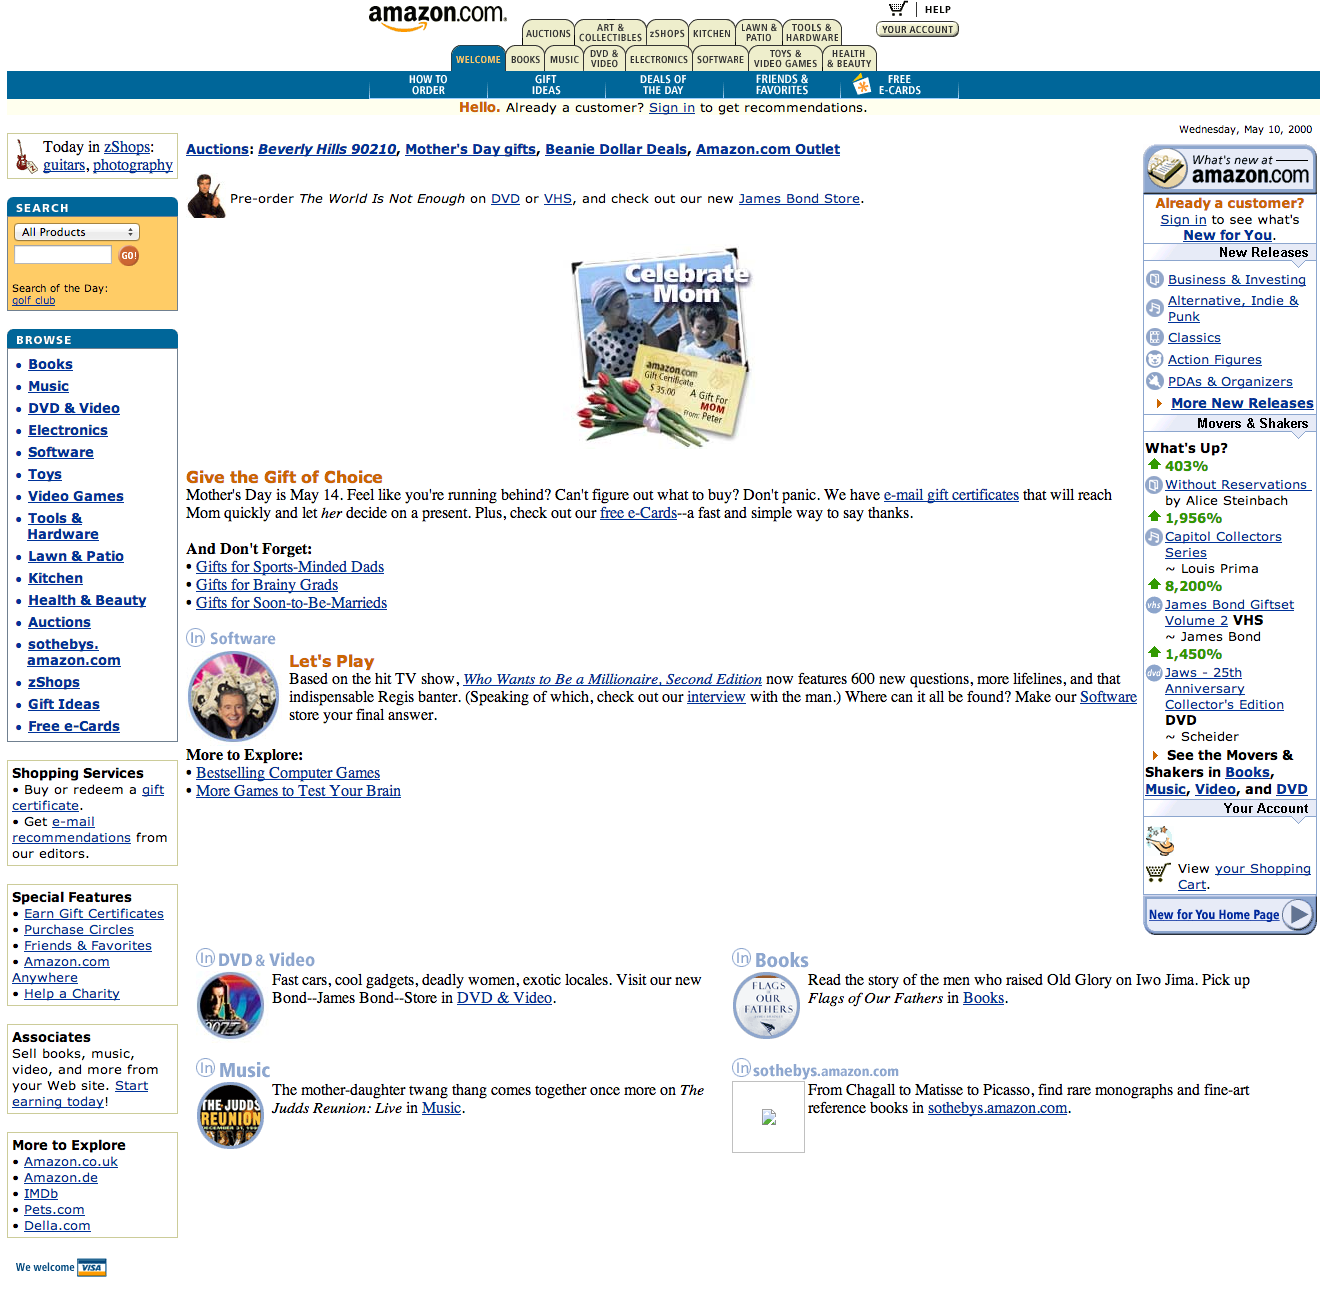
\includegraphics[width=220px]{img/amazon2000}
\end{figure}

\end{frame}

%------------------------------------------------

\begin{frame}
\frametitle{La web hoy}

\textbf{Como son los sitios hoy?}

\begin{itemize}
	\pause \item Sitios complejos
	\pause \item Mucho contenido
	\pause \item Tama�o aproximado de 1800kb %ref 9 de la tesis
\end{itemize}

\end{frame}

%------------------------------------------------

\begin{frame}
\frametitle{Sitio de Amazon, a�o 2014}

\begin{figure}
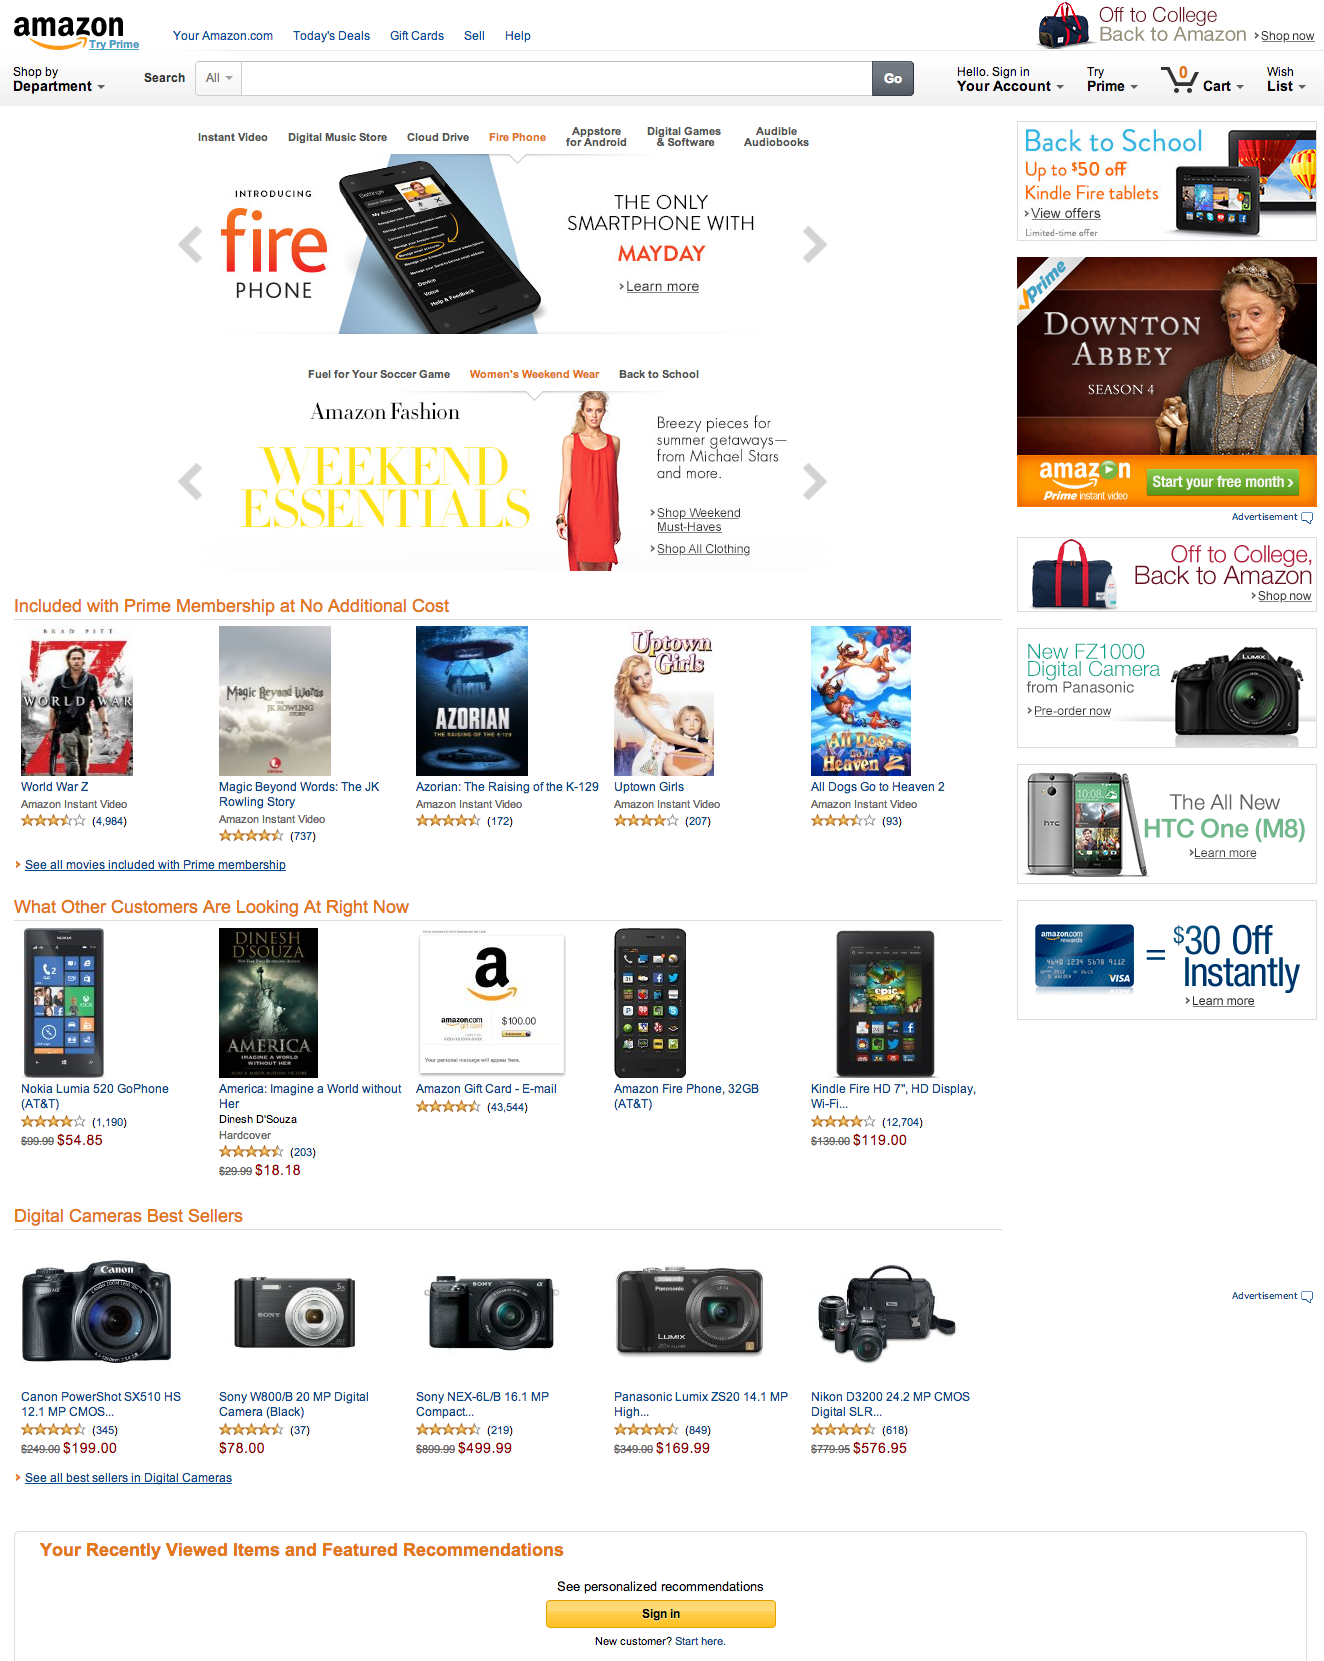
\includegraphics[width=200px]{img/amazon2014}
\end{figure}

\end{frame}

%------------------------------------------------

\begin{frame}
\frametitle{Crecimiento de los usuarios}

\textbf{Aumento de los usuarios globales}

\begin{figure}
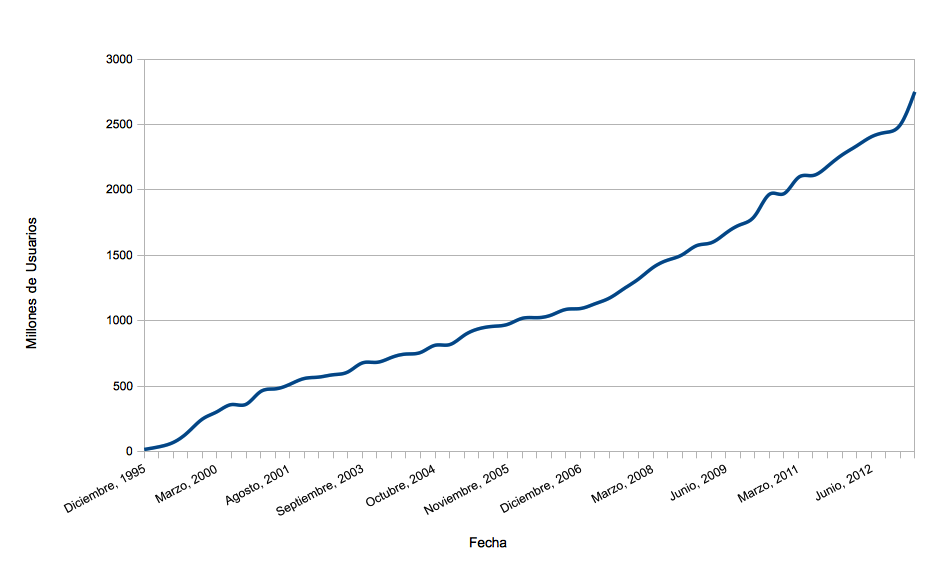
\includegraphics[width=300px]{../tesis/img/grafCrecInternet}
\end{figure}

\end{frame}

%------------------------------------------------
\section{Protocolos}
%------------------------------------------------

\begin{frame}
\frametitle{Definici�n}

\begin{block}{Protocolo}
Un protocolo de comunicaciones define el formato y el orden de los mensajes intercambiados entre dos o m�s entidades que se comunican, as� como las acciones que se toman en la transmisi�n y/o recepci�n de un mensaje u otro evento. %34
\end{block}

\begin{itemize}
	\pause \item Sintaxis
	\pause \item Sem�ntica
	\pause \item Sincronizaci�n
\end{itemize}

\pause \begin{block}{}
\begin{center}\textbf{Las tareas a realizar se dividen en capas}\end{center}
\end{block}

\end{frame}

%------------------------------------------------

\begin{frame}
\frametitle{TCP/IP}
\begin{columns}[c] % The "c" option specifies centered vertical alignment while the "t" option is used for top vertical alignment

\column{.4\textwidth}
\textbf{TCP/IP}
\begin{itemize}
	\pause \item Es el est�ndar de Internet
	\pause \item OSI toma su experiencia 
	\pause \item Dise�o en capas
\end{itemize}

\column{.5\textwidth}
\pause 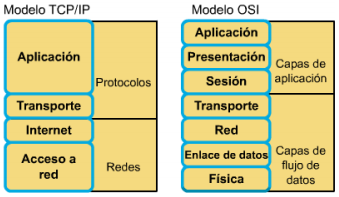
\includegraphics[width=140px]{../tesis/img/tcpiposi}
\end{columns}

\end{frame}

%------------------------------------------------
\subsection{TCP}
%------------------------------------------------

\begin{frame}
\frametitle{TCP}

\begin{block}{TCP (Transport Control Protocol)}
Permite crear conexiones entre hosts para el env�o de flujos de datos.
 \end{block}
 
 \begin{itemize}
	\pause \item Divide los datos en paquetes
	\pause \item Control de recepci�n
	\pause \item Tiempos de espera
	\pause \item Multiplexaci�n
\end{itemize}
 
\end{frame}

%------------------------------------------------

\begin{frame}
\frametitle{TCP}

\begin{block}{}
\begin{center}\textbf{Establecimiento de la conexi�n}\end{center}
\end{block}

\begin{center}
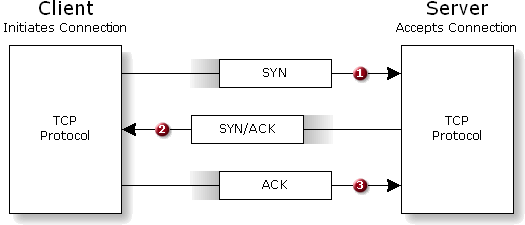
\includegraphics[width=240px]{../tesis/img/threeway}

Three Way Handshake
\end{center}
\end{frame}

%------------------------------------------------
\subsection{HTTP}
%------------------------------------------------

\begin{frame}
\frametitle{HTTP}

\begin{block}{HTTP (HyperText Transfer Protocol)}
Es un protocolo de capa de aplicaci�n que sirve para distribuir informaci�n.
 \end{block}
 
 \begin{itemize}
	\pause \item Primera versi�n en el a�o 1990 (0.9)
	\pause \item Versi�n actual desde el a�o 1999 (1.1)
	\pause \item 1 conexi�n por elemento
	\pause \item Siempre la petici�n la inicia el cliente
\end{itemize}
 
\end{frame}

%------------------------------------------------

\begin{frame}
\frametitle{HTTP}

\begin{center}
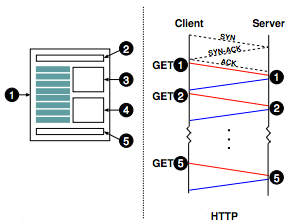
\includegraphics[width=180px]{img/http}%27

Carga de un sitio completo
\end{center}

\end{frame}

%------------------------------------------------
\subsection{HTTPS}
%------------------------------------------------

\begin{frame}
\frametitle{HTTPS}

\begin{block}{HTTPS (HyperText Transfer Protocol Secure)}
Es la versi�n ''segura'' de HTTP, a�ade a este protocolo una capa de cifrado utilizando SSL.
 \end{block}
 
 \begin{itemize}
 	\pause \item Datos protegidos
	\pause \item Los datos viajan encriptados
	\pause \item Necesita establecer una conexi�n segura
\end{itemize}

\end{frame}

%------------------------------------------------

\begin{frame}
\frametitle{HTTPS}

\begin{center}
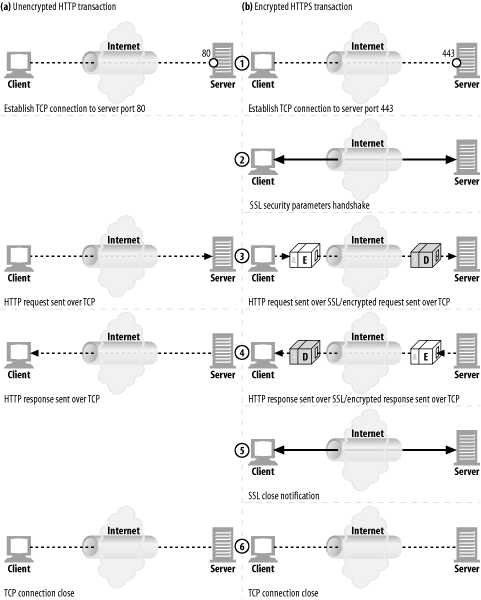
\includegraphics[width=160px]{../tesis/img/httpsConnection}%29

Conexi�n HTTPS
\end{center}

\end{frame}

%------------------------------------------------
\section{Problem�tica de la web}
%------------------------------------------------

\begin{frame}
\frametitle{Problem�tica de la web}

\textbf{Porque es importante mejorar los tiempos de carga de las p�ginas?}

\vspace{1cm}

\begin{columns}[c]
\column{.5\textwidth}
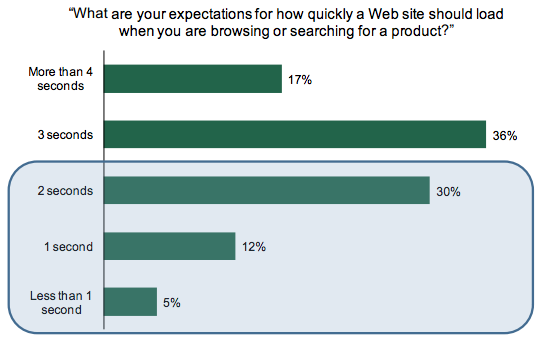
\includegraphics[width=140px]{../tesis/img/aka1}%24
\column{.5\textwidth}
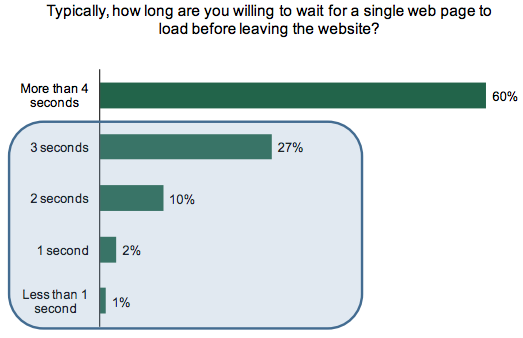
\includegraphics[width=140px]{../tesis/img/aka2}%24
\end{columns}

\begin{center}
Estudio de Akamai
\end{center}

\end{frame}

%------------------------------------------------

\begin{frame}
\frametitle{RTT}

\begin{block}{RTT (Round Time Trip)}
Es el tiempo que demora un paquete en ir del emisor al receptor y volver al emisor nuevamente.
 \end{block}
 
\begin{center}
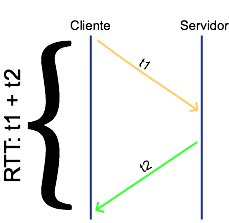
\includegraphics[width=110px]{../tesis/img/rtt}
\end{center}

\end{frame}

%------------------------------------------------

\begin{frame}
\frametitle{Problem�tica de la web}

\textbf{El Ancho de Banda es importante?}

\vspace{1cm}

\begin{columns}[c]
\column{.5\textwidth}
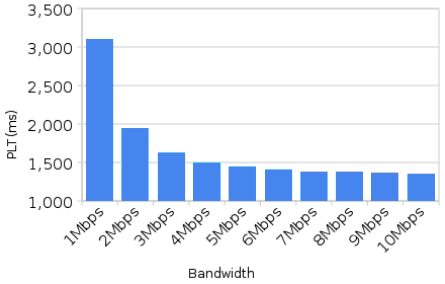
\includegraphics[width=140px]{../tesis/img/belshePLTxBW}%22
\column{.5\textwidth}
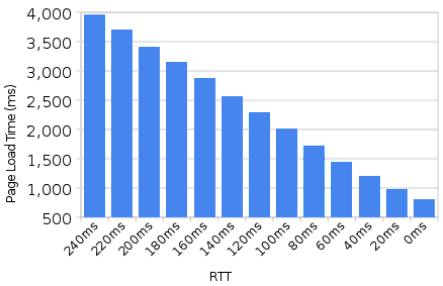
\includegraphics[width=140px]{../tesis/img/belshePLTxRTT}%22
\end{columns}

\begin{center}
Estudio de Mike Belsche
\end{center}

\end{frame}

%------------------------------------------------
\subsection{SPDY}
%------------------------------------------------

\begin{frame}
\frametitle{SPDY}

\begin{block}{SPDY (SPeeDY)}
Es un protocolo experimental desarrollado por Google a mediados del 2009, cuya meta principal es reducir los tiempos de carga de los sitios enfoc�ndose en las limitaciones de HTTP.
\end{block}

\begin{center}
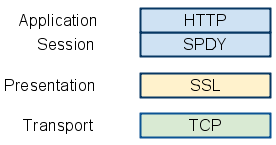
\includegraphics[width=140px]{../tesis/img/capaSPDY}%myracloud.com

Protocolo SPDY
\end{center}

\end{frame}

%------------------------------------------------

\begin{frame}
\frametitle{SPDY}

\textbf{Problemas de HTTP}
 
 \begin{itemize}
 	\pause \item Por cada conexi�n nueva se necesita establecer la conexi�n TCP (RTTs adicionales)
	\pause \item Slow Start de TCP
	\pause \item L�mite de conexiones a un servidor
	\pause \item Domain sharding
\end{itemize}

\end{frame}

%------------------------------------------------

\begin{frame}
\frametitle{SPDY}

\textbf{Que ofrece SPDY?}
 
\begin{columns}[c]
\column{.4\textwidth}
 \begin{itemize}
	\pause \item 1 conexi�n TCP
 	\pause \item Multiplexaci�n
	\pause \item Priorizaci�n
	\pause \item Compresi�n de headers
	\pause \item Server Push
	\pause \item Server Hint
\end{itemize}

\column{.5\textwidth}
\pause 
\includegraphics[width=130px]{img/avionspdy}%27
\end{columns}

\end{frame}

%------------------------------------------------

\begin{frame}
\frametitle{SPDY}

\begin{center}
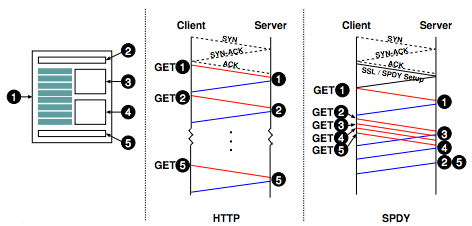
\includegraphics[width=210px]{img/httpspdy}%27

Carga de un sitio completo
\end{center}

\end{frame}

%------------------------------------------------
\section{Proxy} 
%------------------------------------------------

\begin{frame}
\frametitle{Proxy}
?
\end{frame}

%------------------------------------------------
\section{Proxy Adaptativo} 
%------------------------------------------------

\begin{frame}
\frametitle{Proxy Adaptativo}
?
\end{frame}

%------------------------------------------------
\section{Experimentos} 
%------------------------------------------------

\begin{frame}
\frametitle{Experimentos}
?
\end{frame}

%------------------------------------------------
\section{Conclusiones}
%------------------------------------------------

\begin{frame}
\frametitle{Conclusiones}
?
\end{frame}

%------------------------------------------------

\begin{frame}
\Huge{\centerline{FIN}}
\end{frame}

%----------------------------------------------------------------------------------------

\end{document}